\documentclass{article}
\usepackage{hyperref}
\usepackage{amsmath}
\usepackage{graphicx} % Required for inserting images
\usepackage{subcaption} %  for subfigures environments
\usepackage{float}

\title{Photon Mapper}
\author{Javier Sancho Olano \\ \href{mailto:815520@unizar.es}{815520@unizar.es}}
\date{Junio 2024}

\begin{document}

\maketitle

\section{Introducción}
La ecuación de render es una ecuación integral que describe la cantidad de
radiancia emitida de un punto \(\mathbf{x}\) de una superficie hacia una
dirección \(\mathbf{\omega_{o}}\)

\begin{equation}
L_o(\mathbf{x}, \mathbf{\omega_{o}}) = L_e(\mathbf{x}, \mathbf{\omega_{o}}) + \int_{\Omega} L_i(\mathbf{x}, \mathbf{\omega_{i}}) \cdot f_r(\mathbf{x}, \mathbf{\omega_{i}}, \mathbf{\omega_{o}}) \cdot  |\mathbf{n} \cdot \mathbf{\omega_{i}}| \, d\omega_{i}
\end{equation}

\begin{figure}[h]
    \centering
    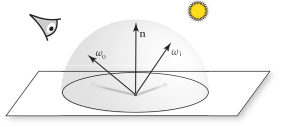
\includegraphics[width=0.6\textwidth]{imgs/rendereq.png}
    \caption{Ilustración del problema de la ecuación de render}
\end{figure}

donde:
\begin{itemize}
  \item \(\mathbf{x}\) es un punto en el espacio
  \item \(\mathbf{\omega_{o}}\) es la direccion de salida
  \item \(\mathbf{n}\) es la normal de la superficie
  \item \(\mathbf{\omega_{i}}\) es la dirección de la radiancia incidente
  \item \(L_o(\mathbf{x}, \mathbf{\omega_{o}})\) es la cantidad de radiancia emitida de un punto \(\mathbf{x}\) de una superficie hacia una dirección \(\mathbf{\omega_{o}}\)
  \item \(L_e(\mathbf{x}, \mathbf{\omega_{o}})\) es la radiancia que la superficie emite en el punto \(\mathbf{x}\), hacia \(\mathbf{\omega_{o}}\)
  \item \(\int_{\Omega} ... \, d\omega_{i}\) es una integral sobre la hemiesfera \(\Omega\)
  \item \(L_i(\mathbf{x}, \mathbf{\omega_{i}}) \) es la radiancia incidente en \(\mathbf{x}\) desde la dirección \(\mathbf{\omega_{i}}\)
  \item \(f_r(\mathbf{x}, \mathbf{\omega_{i}}, \mathbf{\omega_{o}}) \) es la BTDF, la proporción de radiancia reflejada hacia \(\mathbf{\omega_{o}}\) desde \(\mathbf{\omega_{i}}\) en el punto \(\mathbf{x}\)
  \item \(|\mathbf{n} \cdot \mathbf{\omega_{i}}|\) a.k.a \(\cos\theta_{i}\) es el factor que ajusta la contribución de la radiancia incidente respecto a \(\mathbf{\omega_{i}}\)
\end{itemize}

El algoritmo \textit{photon mapper} es un algoritmo de dos pasos que resuelve
esta ecuación. En el primer paso, se generan fotones que se trazan en la escena
desde las fuentes de luz. En el segundo paso, se trazan rayos desde la cámara y
al intersectar con la escena se calcula la radiancia en ese punto usando los
fotones generados en el paso anterior.

Con un número grandede fotones, tras el primer paso tendremos toda las escena
cubierta por fotones y por lo tanto, los fotones alrededor de un punto dado
darán una buena estimación de la radiancia incidente en ese punto.

La radiancia en un punto se define como:
\begin{equation} 
  L_i(\mathbf{x}, \mathbf{\omega_{i}}) = \frac{d^{2}\phi_{i}(\mathbf{x}, \mathbf{\omega_{i}})}{\cos\theta_{i} \: d\omega_{i} \: dA_{i}},
\end{equation}

dónde:
\begin{itemize}
  \item \(\mathbf{x}\) es un punto en el espacio
  \item \(\omega_{i}\) es la dirección de la radiancia incidente
  \item \(\phi_{i}(\mathbf{x}, \mathbf{\omega_{i}})\) es el flujo de los fotones en el punto \(\mathbf{x}\) en la dirección \(\mathbf{\omega_{i}}\)
  \item \(\cos\theta_{i}\) es el factor de corrección de la radiancia incidente
  \item \(A_{i}\) es el área de la superficie donde incide la radiancia
\end{itemize}

Con esto, podemos reescribir la ecuación de render como (omitiendo la radiancia
emitida):
\begin{equation}
\begin{split}
  L_o(\mathbf{x}, \mathbf{\omega_{o}}) & = \int_{\Omega} \frac{d^{2}\phi_{i}(\mathbf{x}, \mathbf{\omega_{i}})}{\cos\theta_{i} \: d\omega_{i} \: dA_{i}} \cdot f_r(\mathbf{x}, \mathbf{\omega_{i}}, \mathbf{\omega_{o}}) \cdot  |\mathbf{n} \cdot \mathbf{\omega_{i}}| \, d\omega_{i} \\
                                       & = \int_{\Omega} \frac{d^{2}\phi_{i}(\mathbf{x}, \mathbf{\omega_{i}})}{dA_{i}} \cdot f_r(\mathbf{x}, \mathbf{\omega_{i}}, \mathbf{\omega_{o}}) \\
\end{split}
\end{equation}

El flujo \(\phi_{i}\) se aproximará usando los \(n\) fotones más cercanos a
\(\mathbf{x}\) y cada fotón \(p\) tiene un flujo asociado \(\phi_{p}\).
\(\Delta A\) es el área de la superficie que cubre los \(n\) fotones, si \(r\)
es la distancia entre \(\mathbf{x}\) y el fotón más lejano, entonces
\(\Delta A = \pi r^{2}\). Entonces, aproximaremos la ecuación de render como:

\begin{equation}
\begin{split}
  L_o(\mathbf{x}, \mathbf{\omega_{o}})  & \approx \sum_{p=1}^{n} \frac{\phi_{p}}{\Delta A} \cdot f_r(\mathbf{x}, \mathbf{\omega_{p}}, \mathbf{\omega_{o}}) \\
                                        & \approx \frac{1}{\pi r^{2}} \sum_{p=1}^{n} \phi_{p} \cdot f_r(\mathbf{x}, \mathbf{\omega_{p}}, \mathbf{\omega_{o}})
\end{split}
\end{equation}

\section{Iluminación directa}
Vamos a comparar la iluminación directa con y sin next-event estimation. Para
ello, usaremos la escena \textit{Cornell Box} con dos esferas de material
completamente difuso y una luz puntual. En la figura \ref{fig:direct} se muestra
la escena renderizada con iluminación directa y en la figura
\ref{fig:direct_nee} se muestra la escena renderizada con iluminación directa y
next-event estimation.

\begin{figure}
\begin{subfigure}[h]{0.4\linewidth}
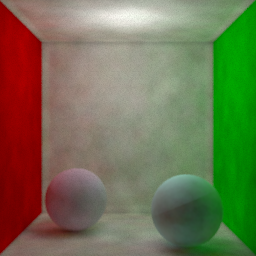
\includegraphics[width=\linewidth]{imgs/pml.png}
\caption{Iluminación directa sin next-event estimation}
\end{subfigure}
\hfill
\begin{subfigure}[h]{0.4\linewidth}
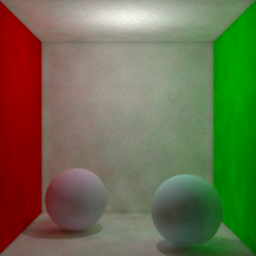
\includegraphics[width=\linewidth]{imgs/pmdl.png}
\caption{Iluminación directa con next-event estimation}
\end{subfigure}
\caption{Cornell Box con 2 esferas difusas}
\end{figure}

La principal diferencia que observames entre las dos imagenes son las
\textbf{\textit{hard shadows}}.

El cálculo de la radiancia incidente genera una estimación sesgada. Esta
situación se ilustra en la Figura 3, en un punto de transición, la radiancia
incidente se estima con los fotones más cercanos, tanto en un lado de la sombra
como en el otro. Esto suaviza la transición.

Por este motivo, el efecto de \textit{soft shadows} será muy fácil de obtener
con el photon map.

Mediante el uso de \textit{next-event estimator} es posible obtener una estimación no sesgada de la radiancia directa incidente calculando TODO

\begin{figure}
\begin{subfigure}[h]{0.4\linewidth}
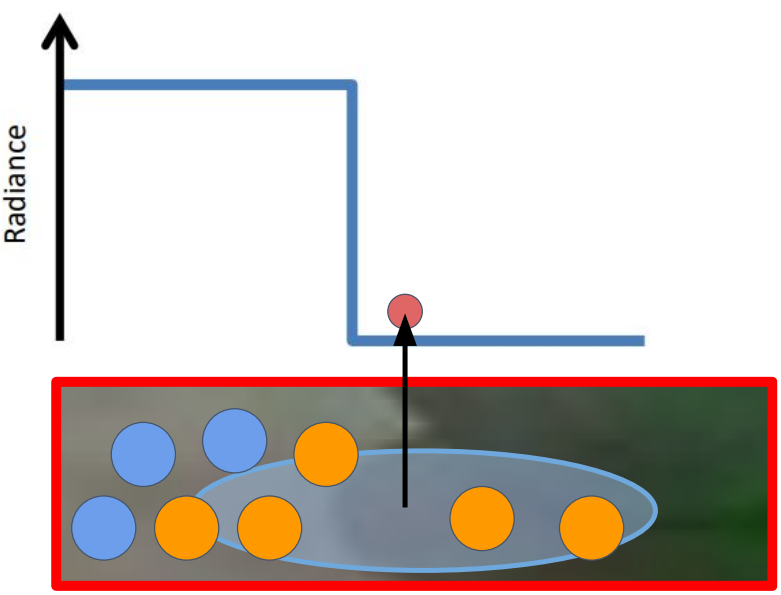
\includegraphics[width=\linewidth]{imgs/rad1.png}
\end{subfigure}
\hfill
\begin{subfigure}[h]{0.4\linewidth}
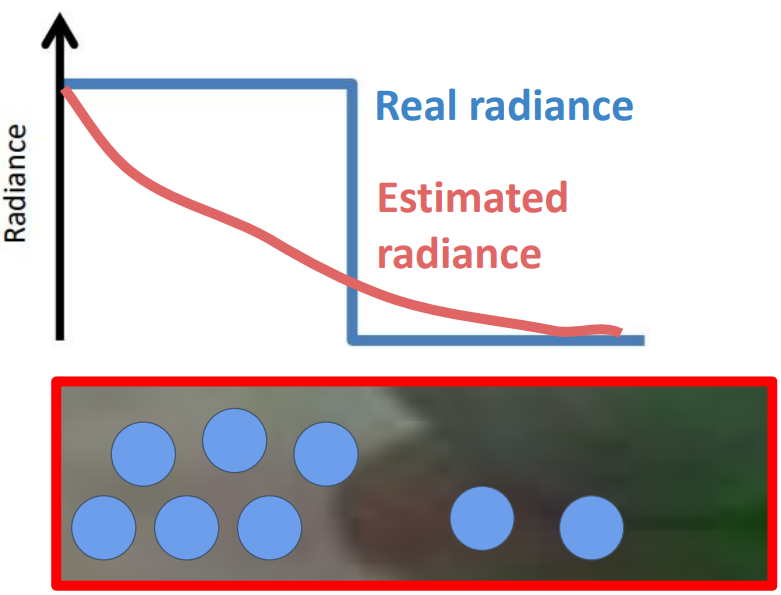
\includegraphics[width=\linewidth]{imgs/rad2.png}
\end{subfigure}
\caption{Ilustración de la estimacion sesgada de la radiancia incidente. Tomada de las diapositivas del laboratorio.}
\end{figure}

\section{Efectos de las BSDFs delta}
Para analizar los efectos de las BSDFs delta, vamos a renderizar la escena
\textit{Cornell Box} con una esfera de material plastico (difuso + especular),
otra esfera con un material de cristal (transmisiva y especular) y una luz
puntual.

\begin{figure}[H]
\centering
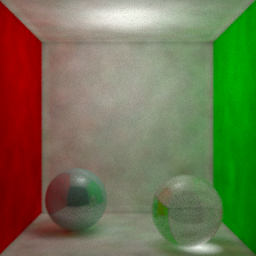
\includegraphics[width=0.6\linewidth]{imgs/pm_delta1.png}
\caption{Cornel Box con una esfera de cristal y otra de plastico}
\end{figure}

En primer lugar, una BSDF delta solo dispersaba la radiación en una dirección.
Por lo que \(f_r(\mathbf{x}, \mathbf{\omega_{i}}, \mathbf{\omega_{o}})\) será 0
para cualquier \(\mathbf{\omega_{i}}\) distinto de su único vector posible.
Sabiendo esto, el término
\( f_r(\mathbf{x}, \mathbf{\omega_{p}}, \mathbf{\omega_{o}}) \) de la ecuación 4
será 0 para cualquier fotón que no haya sido dispersado por la BSDF delta, que
es imposible TODO EXPLICAR MEJOR

En la primera pasada del algoritmo, cuando un rayo se encuentre con una BSDF
delta, seguirá el camino pero no guardará el fotón.

Por lo que todos los efectos de refracción y reflexión de la esfera de cristal
se computarán desde la parte de ray tracing.

Por otro lado y por la misma razon, las causticas, colorbleeden TODO EXPLICXAR MEJOR

TODO QUIZAS AQUI TAMBIEN SE PUEDE HABLAR DE QUE EL NEE SE HACER EN LA PARTE DE RAY TRACING?? TODO: hard y soft shadows/? decir alhgo?

Which of the lighting and appearance effects come from photon mapping? Which of those effects come
from the ray tracing part of the algorithm?

\section{Resultados obtenidos}

Antes de empezar, vamos a analizar como el numero de fotones y el numero de vecinos afectan en el resultado analiticamente.
Dado un numero de fotones \(N\), un "grado de infinitud" \(\alpha\) y las ecuaciones 3 y 4, podemos ver que:

\begin{equation}
\begin{split}
\lim_{N\to\infty} \sum_{p=1}^{\lfloor N^{\alpha}\rfloor} \frac{\phi_{p}}{\Delta A} \cdot f_r(\mathbf{x}, \mathbf{\omega_{p}}, \mathbf{\omega_{o}}) &= \int_{\Omega} \frac{d^{2}\phi_{i}(\mathbf{x}, \mathbf{\omega_{i}})}{dA_{i}} \cdot f_r(\mathbf{x}, \mathbf{\omega_{i}}, \mathbf{\omega_{o}}) \\
  &= L_o(\mathbf{x}, \mathbf{\omega_{o}})
\end{split}
\end{equation}

donde \(\lfloor N^{\alpha} \rfloor\) es el numero de vecinos que se usaran para estimar la radiancia incidente. Este numero nos permite justificar que el numero de vecinos sera infinitamente mas pequeno que el numero de fotones.
De esta forma obtenemos que la estimacion de la radiancia sera arbitrariamente precisa si el numero de fotones tiende a infinito.

En la practica esto no es posible, por lo que debemos tener un compromiso entre calidad de imagen y coste computacional. Vamos a ver como afectan estos parametros en la calidad de la imagen:

\subsection{Número de fotones}
Dejando fikado el numero de vecinos, aumentar el numero de fotones provocara,
en primer lugar que los fotones esten mas repartidos por la escena y como resultado
que la estimacion de la radiancia incidente sea mas precisa. tal y como eq 5 y decir nose de convergendia
FIGURA 5
Naturalmente, el coste computacional aumentara...
TODO

\begin{figure}
\begin{subfigure}[h]{0.22\linewidth}
\includegraphics[width=\linewidth]{imgs/1k10kv.png}
\caption{N=1000. Patron similar a una partición de Voronoi debido a la baja cantidad de fotones y un radio alto.}
\end{subfigure}
\hfill
\begin{subfigure}[h]{0.22\linewidth}
\includegraphics[width=\linewidth]{imgs/1k10k.png}
\caption{N=1000. Esta vez con un radio mas bajo se puede observar la distribución de los (pocos) fotones.}
\end{subfigure}
\hfill
\begin{subfigure}[h]{0.22\linewidth}
\includegraphics[width=\linewidth]{imgs/10k10k.png}
\caption{N=10,000.}
\end{subfigure}
\hfill
\begin{subfigure}[h]{0.22\linewidth}
\includegraphics[width=\linewidth]{imgs/100k10k.png}
\caption{N=100,000.}
\end{subfigure}

\caption{Cornell Box con k=10 y diferentes valores de N}
\end{figure}

\subsection{Número de vecinos}
Fijando el numero de fotones, aumentar el numero de vecinos provocara que la estimacion de la radiancia incidente sea mas precisa. Sin embargo, si el numero de vecinos es muy grande, el coste computacional sera muy alto. Como se puede ver en la equciaon

TODO

\begin{figure}
\begin{subfigure}[h]{0.32\linewidth}
\includegraphics[width=\linewidth]{imgs/100k200k.png}
\caption{k=200.}
\end{subfigure}
\hfill
\begin{subfigure}[h]{0.32\linewidth}
\includegraphics[width=\linewidth]{imgs/100k1000k.png}
\caption{k=1,000.}
\end{subfigure}
\hfill
\begin{subfigure}[h]{0.32\linewidth}
\includegraphics[width=\linewidth]{imgs/100k2000k.png}
\caption{k=2,000.}
\end{subfigure}

\caption{Cornel Box con N=100,000 y diferentes valores de k}
\end{figure}

\section{Extensiones}
\subsection{Kernels}

Si el radio de busqueda es muy grande, la estimacion de la radiancia puede ser imprecisa provocando que un aspecto borroso como se puede observar en la Figura 7 a, a su vez, esto proboca que las cuasticas noseque porque nosecuantas TODO

Para reducir este efecto, usamos los kernels. Los kernels funcionan asignado un peso a cada fotón en función de su distancia a \(\mathbf{x}\). Los kernels mas comunes son el kernel gaussiano y el kernel conico. TODO wp

\begin{equation}
L_o(\mathbf{x}, \mathbf{\omega_{o}}) \approx \sum_{p=1}^{n} \phi_{p} \cdot f_r(\mathbf{x}, \mathbf{\omega_{p}}, \mathbf{\omega_{o}}) \cdot w_p
\end{equation}


\begin{figure}
\begin{subfigure}[h]{0.32\linewidth}
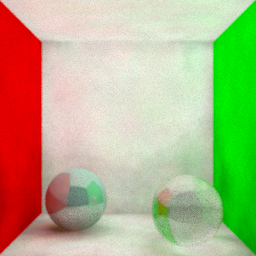
\includegraphics[width=\linewidth]{imgs/box.png}
\caption{Box kernel}
\end{subfigure}
\hfill
\begin{subfigure}[h]{0.32\linewidth}
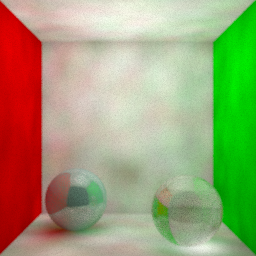
\includegraphics[width=\linewidth]{imgs/cone1.png}
\caption{Cone kernel}
\end{subfigure}
\hfill
\begin{subfigure}[h]{0.32\linewidth}
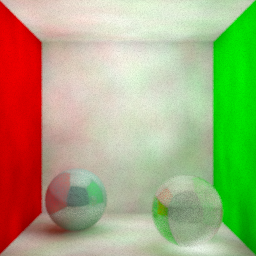
\includegraphics[width=\linewidth]{imgs/gaussian.png}
\caption{Gaussian kernel}
\end{subfigure}
\caption{Usar kernels para mejorar la estimacion de la radiancia}
\end{figure}

\end{document}
